% Tento soubor nahraďte vlastním souborem s obsahem práce.
%=========================================================================
% Autoři: Michal Bidlo, Bohuslav Křena, Jaroslav Dytrych, Petr Veigend a Adam Herout 2019
\chapter{Úvod}

Cieľom tejto bakalárskej práce je návrh architektúry a následná implementácia aplikácie určenej na extrakciu dát z webových stránok. V dnešnej dobe je pojem extrakcia dát používaný stále častejšie v spojitosti práve s webovými technológiami a webom samotným. Je to tak práve preto, že sa internet ako taký, a hlavne jeho obsah v podobe webových stránok, neustále rozširuje. Objem dát ktoré sa na webe nachádza sa zväčšuje neúprosnou rýchlosťou, a preto je zber údajov z rôznych webstránok stále zložitejší. A to nielen čo sa zložitosti štruktúry webu týka, ale vzhľadom na veľký počet webov sa zvyšuje aj časová náročnosť analýzy a následnej extrakcie dát.

Práve pre spomínanú expanziu internetu sa tejto téme venuje čoraz viac spoločností so snahou uľahčiť prístup k web scrapingu pre každodenných užívateľov. Pre neustáli vývoj webu je avšak nutné vyvíjať aj aplikácie, ktoré sú na extrakciu určené. 

Pri rozlišovaní takýchto aplikácií sa berie na vedomie hlavne požadovaný vstupný formát a jeho zložitosť, požadovaný výstupný formát a jeho využiteľnosť v praxi, a v neposlednom rade rýchlosť aplikácie z pohľadu extrakcie dát. 

Táto práca je zameraná hlavne na časť týkajúcu sa požadovaného vstupu aplikácie, kde je za cieľ požadovaný jednotný vstup vo formáte JSON. Tento vstup pozostáva z adries webových stránok, dátových typov, rozloženia objektov na webstránke, a požadovaných názvov extrahovaných informácií. Aplikácia sa následne pozerá na každú stránku zvlášť a určí výsledné údaje na základe poskytnutých relevantných informácií o štruktúre. Týmto spôsobom je možné definovať jeden vstup raz, a použiť ho na viaceré webové dokumenty bez nutnosti ďalšieho zásahu.

Prvá časť práce sa v kapitole \ref{aktualny_pristup} zaoberá aktuálnym prístupom k problematike, ako sa web scraping využíva v súčasnosti, aké sú štandardy a dostupné technológie, a porovnanie týchto prístupov z hľadiska využiteľnosti.

V druhej časti tejto práce sú v kapitole \ref{Technologie} popísané technológie ktoré je treba brať v úvahu pri návrhu, tvorbe a analýze aplikácie určenej na extrakciu dát. Jedná sa hlavne o technológie ktoré sa stali základným kameňom navrhnutej aplikácie, a o technológie na ktorých aplikácia stavia.

Kapitola 4 sa zameriava na analýzu a návrh architektúry aplikácie. Je založená na analýze špecifikácie a požiadavkov aplikácie, a popisuje postup návrhu aplikácie.

V 5. kapitole sú popísané jednotlivé detaily implementácie riešenia, a hlavná logika aplikácie.

6. kapitola sa následne venuje testovaní aplikácie za pomoci niekoľkých datasetov, a následnej analýze a vyhodnotení výsledkov ktoré aplikácia dosiahla.


\chapter{Aktuálny prístup k problematike Web Scrapingu}
\label{aktualny_pristup}

V tejto kapitole sú uvedené a popísané aktuálne prístupy ktoré sa používajú na extrakciu dát z webových dokumentov. Takáto extrakcia môže prebiehať online alebo offline, v závislosti na tom aké dáta a za akým cieľom chceme extrahovať.

Web scrapingu ako takému sa v súčasnosti venuje stále viac a viac spoločností, a preto nieje prekvapením že sa rozširujú nielen možnosti web scrapingových aplikácií, ale aj prístup takýchto aplikácií k priamej extrakcii dát.

Zároveň sa rozširuje pole pôsobnosti, a možnosti využitia takto extrahovaných dát. Preto je táto kapitola určená hlavne rozboru týchto metód. Poznatky získané z tohto rozboru zároveň pomôžu určiť smer ktorým sa návrh a vývoj aplikácie môžu uberať. 

\section{Web scraping}

Web scraping je jednou z foriem získavania údajov z webových stránok. Takéto získavanie údajov je možné buď priamo - \textit{World Wide Web} za pomoci \textit{Hypertext Transfer Protokolu}, alebo pomocou webového prehliadača (napr. Google Chrome). Za web scraping sa dá považovať aj manuálny zber dát za využitia ľudskej sily, ale všeobecne sa tým myslí využitie dedikovaného počítača ktorý túto prácu automatizuje. Tu sa môže jednať napríklad o jednoduché kopírovanie dát, alebo zložitejšie generovanie výstupných štruktúr napríklad vo formáte JSON.

Automatizované získavanie informácií z webu sa dostalo do vývoja krátko po zavedení World Wide Web. Kvôli neustálemu vývoju technológií je však vo vývoji doteraz, a jeho možnosti sa neustále rozširujú. Prvé formy automatizovaných web scraperov boli určené primárne pre tvorbu databázy vyhľadávacieho indexu pre vývoj World Wide Web Vyhľadávače. Za jeden z prvých takýchto scraperov je preto považovaný World Wide Web Wanderer, ktorý bol vyvinutý v roku 1993 za účelom zmerania veľkosti celého internetu, a neskôr na jeho priamu indexáciu. \cite{wiki:Web_scraping}

\section{Súčasné postupy}

Existujú rôzne prístupy k danej problematike, kde rozdiely sú jednoznačné hlavne pri spôsobe a type analýzy a extrakcie finálnych dát. Hlavným cieľom pri tvorbe aplikácie na takúto extrakciu dát je užívateľská prívetivosť, a jednoduchosť definovania vstupných požiadavkov. Postup ktorý aplikácie na extrakciu dát využívajú je prevažne rovnaký, a skladá sa z troch primárnych krokov:
\begin{enumerate}
  \item{Odoslanie GET požiadavku na webový server a následné obdržanie odpovedi}
  \item{Analýza extrahovaného HTML kódu na základe stromovej štruktúry}
  \item{Použitie zvoleného postupu na extrakciu dát a spracovanie hľadaného obsahu}
\end{enumerate}

Tieto kroky sú potom pri každej aplikácií mierne prispôsobené určeniu a typu implementácie. \cite{online:how_does_scraping_work}

\begin{figure}[hbt]
	\centering
	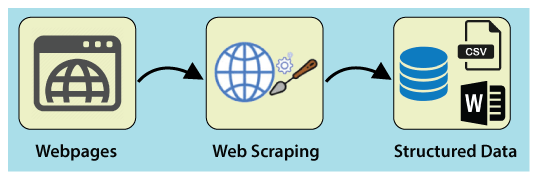
\includegraphics[width=0.7\textwidth]{obrazky-figures/web-scraping-using-python.png}
	\caption{Všeobecný postup ktorým sa aplikácia typu web scraper riadi. Prevzaté z Javatpoint \cite{WebScrap}}
	\label{WebScrap_img}
\end{figure}

\bigskip

Medzi najpopulárnejšie web scrapery patria aplikácie s jednoduchou point-and-click politikou, kde používateľ po inštalácií takejto aplikácie jednoducho zvolí webové dokumenty z ktorých chce extrakciu prevádzať, a následne interaktívne vyznačí dáta ktoré ho zaujímajú. Pre užívateľov ktorý nemajú príliš veľké skúsenosti s informačnými technológiami a nechcú platiť za túto službu nemalé peniaze rôznym korporáciám je to skrátka jediná možnosť.

\bigskip

Spomínaný prístup má samozrejme svoje výhody, medzi ktoré sa radí najmä spomínaná užívateľská prívetivosť a relatívne nízka cena, avšak v prípade potreby automatizácie takejto činnosti existujú na trhu lepšie riešenia. V prípade že je potrebná vysoká automatizácia, alebo sa jedná o veľké množstvo dát a stránok ktoré sú na extrakciu určené, je výhodnejšie použiť aplikáciu ktorá je ladená skôr na tento spôsob. Pri firmách ktoré sa venujú extrahovaniu údajov z webových stránok na profesionálnej úrovni sa počet prenesených dát v súčasnosti pohybuje už v petabajtoch, a počet extrahovaných webových stránok sa pohybuje v miliardách mesačne na jednu takúto firmu. 

Pri takto veľkých číslach narážajú spomínané firmy na rôzne problémy, ktoré rádový používateľ web scrapingovej aplikácie riešiť nemusí. Medzi takéto problémy sa radia v neposlednom rade napríklad:
\begin{itemize}
    \item {Náročnosť na hardvérový čas}
    \item {Limitovanie počtu možných GET dotazov}
    \item {Veľká diverzifikácia architektúry webových stránok}
    \item {Objem dát potrebný na prenesenie údajov a následné uloženie extrahovaných údajov}
\end{itemize}

Príklad ako sa takýmto problémom brániť alebo im priam predchádzať je v prípade limitovania počtu možných GET dotazov na jednu webovú stránku meniť IP adresy z ktorých sú GET dotazy odosielané. Ani to však nie vždy môže byť riešením, keďže stránky v dnešnej dobe môžu využívať rôzne ochrany proti web scrapingu, ako napríklad priamu detekciu človeka od robota alebo tzv. CAPTCHA\footnote{Completely Automated Public Turing test to tell Computers and Humans Apart.} .\cite{JanCurna:online} 

Web scraping má teda svoje výhody, ale aj nevýhody. Tieto sú popísané podrobnejšie v nasledujúcej časti tejto kapitoly.

\section{Výhody, nevýhody, a využitie web scrapingu}

Web scraping má v súčasnosti viac možností a oblastí využitia ako tomu bolo v minulosti. Toto je dané hlavne neustálim rozširovaním sa internetu ako celku. V počiatkoch internetu sa aplikácie typu web scraper nazývali skôr crawler, a využívali prevažne na indexáciu obsahu, a nie na zber, extrakciu a analýzu dát tak ako je tomu teraz. 

Web scraper je ale aplikácia ktorá je založená presne na tých fundamentálnych základoch ako spomínaný crawler, s jediným rozdielom a to tým, že jeho úlohou je zber dát. Takýto zber môže prebiehať napríklad kopírovaním dát do databázy. V mnohých prípadoch sú aplikácie typu scraper využívané veľkými korporáciami ako napríklad Microsoft, Amazon alebo Google na cielenie zobrazovaných reklám tak, aby boli pre užívateľa ako jednotlivca relevantné.\cite{online:how_does_scraping_work}

\bigskip

Jednotlivé prípady využitia takejto aplikácie sa neustále rozširujú, obecne ale platí že jeho využitie spadá do nasledovných kategórií:

\begin{itemize}
    \item {Monitorovanie ceny produktov}
    \item {Získavanie údajov o nových produktoch na trhu}
    \item {Analýza konkurencie}
    \item {Evidovanie údajov o konkrétnej doméne podľa druhu záujmu}
    \item {Monitorovanie ceny leteniek}
\end{itemize}

A mnohé ďalšie prípady. Údaje extrahované touto metódou môžu byť následne využité na širšie pochopenie vývoja udalostí napríklad na trhu, alebo u konkurencie.

Web scraping má teda jasné výhody čo sa kolekcie dát týka. Patria medzi ne už spomínané monitorovanie konkurencie, cien produktov a analýza rôznych dát. V neposlednom rade ale treba zmieniť aj výhody z pohľadu technológie samotnej. Medzi ne patria napríklad:

\begin{itemize}
    \item {Rýchlo sa rozvíjajúce technológie}
    \item {Automatizovanie monotónnych činností}
    \item {Zber obsiahleho množstva dát, ktorý by bol manuálne nemožný}
    \item {V porovnaní s manuálnym zberom dát exponenciálne rýchlejšie výsledky}
\end{itemize}

Každá technológia a jej využitie má však aj svoje nevýhody. V porovnaní s manuálnym zberom dát, ktoré môže byť rozumné ak sa jedná o ojedinelú prípadne unikátnu udalosť, kedy je takýto zber potrebné vykonať jeden krát za dlhé obdobie, sa tvorba alebo priame využitie web scrapera očakáva až v prípade že sa daná akcia musí vykonávať automatizovane a v určitých časových intervaloch. \cite{WebScrap}

V takom prípade je potreba zvážiť aj rôzne prvky pri nielen prevádzke, ale aj samotnom vytváraní a následnom používaní web scrapera. Medzi najhlavnejšie nevýhody sa preto radí najmä:

\begin{itemize}
    \item {Nutná znalosť kódu a programovania}
    \item {IP Detekcia a CAPTCHA}
    \item {Ku každej stránke je potreba pristupovať individuálne}
\end{itemize}

Zároveň treba spomenúť fakt, že dynamické stránky môžu meniť svoju štruktúru, a preto nemôžme zabúdať na údržbu web scrapera nielen z pohľadu úrovne bezpečnosti programu, ale aj z pohľadu údajov ktoré web scraper prijíma. V prípade že webová stránka zmení štruktúru tak, že aktuálna konfigurácia web scrapera nedokáže pokračovať v extrahovaní údajov tak ako predtým, je potrebné v mnohých prípadoch stránku znova analyzovať, a v prípade že je web scraper neschopný efektívne využiť algoritmy ktoré v minulosti fungovali, v niektorých prípadoch aj dodatočne zanalyzovať prístupy web scrapera a upraviť jeho logiku tak, aby mohol v extrahovaní pokračovať.

\section{Metódy využívané v súčasnosti}

V prípade že nás zaujíma len priama extrakcia dát, v dnešnej dobe je na výber z mnohých aplikácií ktoré sú pripravené na použitie, a tak nieje treba programovať aplikácie znova. Každá má však svoje vlastné postupy pri extrakcii, a z toho plynie fakt že nie každá takáto aplikácia dokáže splniť požadované zadanie. Medzi najznámejšie aplikácie v tomto odvetví však patria hlavne:

\begin{itemize}
    \item {Scrapping-bot}
    \item {Octoparse}
    \item {Import.io}
    \item {Dexi.io}
    \item {Outwit}
\end{itemize}

V niektorých prípadoch nám stačí jednoduché rozšírenie do prehliadača (napr. Web Scraper\footnote{\url{https://webscraper.io/}}) ktoré sú samozrejme efektívne hlavne pri menšom počte webstránok a dát určených na scraping. \cite{WebScrap}

\bigskip

Pokiaľ však chceme vytvoriť vlastný program alebo aplikáciu typu web scraper, je potrebné rozlišovať na úrovni technológií dostupných pri programovaní. V prvom rade je treba vziať do úvahy programovací jazyk. V takom prípade je na výber rovno z niekoľko volne dostupných programovacích jazykov. Medzi dva najpopulárnejšie však patria hlavne Python, a Node.js. Každý má však znova svoje výhody a nevýhody, a preto je treba zvážiť na aké účely bude web scraper používaný. Vo všeobecnosti je populárnejší práve prvý spomínaný Python, vďaka jeho popularite z pohľadu jednoduchosti písania čistého kódu, komunity, a podpory ktorá je mu venovaná. Python ponúka veľké množstvo frameworkov, z ktorých tie najpopulárnejšie zahŕňajú hlavne Selenium\footnote{\url{https://www.selenium.dev/}} a Scrapy\footnote{\url{https://scrapy.org/}}, ktoré som samozrejme zohľadnil pri výbere vhodného frameworku na vytvorenie web scrapera.

Na druhej strane Node.js stavia na základoch Javascriptu, ktorý je vyvíjaný priamo pre prácu s web stránkami. Kým Python je lepší čo sa týka podpory a rozšírenosti frameworkov, Javascript má výhodu v lepšej integrácií nielen s webovými stránkami ako takými, ale aj s webovými prehliadačmi samotnými. Python v mnohých prípadoch vyžaduje driver na komunikáciu s prehliadačom, a podpora dynamických stránok je znova jednoznačne lepšia pomocou Javascriptu, práve kvôli jeho spomínanej lepšej integrácií a faktom, že Javascript je jednou z hlavných súčastí dynamických moderných webových stránok. Javascript je jednou z hlavných prvkov modernej webovej stránky, ktorá sa skladá ešte z HTML a CSS. Jeho úlohou je hlavne vytváranie dynamického obsahu vytvárajúceho dojem že webová stránka s užívateľom interaguje. Vo väčšine prípadov beží iba na strane klienta, takže dynamickosť samotná nezaťažuje server. Zároveň je v mnohých prípadoch využívaná asynchrónnosť\footnote{Asynchrónnosť znamená v tomto prípade neblokovanie prehliadačových prostriedkov a načítavanie obsahu za behu webstránky.} tohto programovacieho jazyka, na zlepšenie odozvy a interakcie. Práve tento fakt sa stáva rozdielovým faktorom pri extrakcii dát z webových stránok, keďže obsah webovej stránky sa v mnohých prípadoch môže načítavať asynchrónne a nezávisle od ostatných častí webu. Z môjho vlastného rozboru a výskumu som zistil, že dynamickosť a asynchrónnosť stránok je prvok ktorý je lepšie zvládaný za pomoci Javascriptu. \cite{The5Best}\cite{Javascript}

\bigskip

Rozhodnutie používať Javascript som učinil zároveň s predpokladom využitia jedného z jeho volne dostupných frameworkov, a zároveň som zohľadnil svoje predošlé skúsenosti práve so spomínaným jazykom. K tomuto rozhodnutiu prispel aj fakt, že v dnešnej dobe je dynamika stránok takmer štandard, a tu hrá úloha Javascriptu veľkú rolu. V procese výberu frameworku som zohľadňoval hlavne integráciu daného frameworku s prehliadačom, výbornú podporu dynamických stránok a asynchrónnosť ktorá je pri takejto aplikácii kľúčová.

Ako prvý framewrok spomeniem určite Apify SDK, za ktorým stojí Česká firma Apify Technologies\footnote{{\url{https://apify.com/}}}.\cite{JanCurna:online} Práve Apify ma totiž inšpirovalo v rôznych odvetviach vývoja. Medzi najznámejšie technológie ktoré používajú Javascript patria najmä:

\begin{itemize}
    \item {Apify SDK}
    \item {Puppeteer}
    \item {Cheerio}
\end{itemize}

Z pomedzi týchto technológií ktoré zdieľajú niektoré základné funkcie bola na zostavenie výslednej aplikácie použitá technológia Puppeteer. Puppeteer je zároveň jedna z technológií využívaných práve spomínanou Českou firmou Apify. 

V porovnaní s technológiou Cheerio má Puppeteer svoje výhody. V niektorých faktoroch vyhráva ale aj Cheerio, a preto je treba zvážiť hlavne nasledovné:

\begin{itemize}
    \item {Možnosť scrapingu dynamických stránok}
    \item {Funkcionality a možnosti}
    \item {Kompatibilita webových technológií}
    \item {Rýchlosť analýzy a extrakcie}
\end{itemize}

V prvom rade treba zvážiť aktuálnu situáciu a technológie ktoré sa na webe vyskytujú. 95\% webových stránok v súčasnosti používa Javascript, takže predpoklad že moderné weby budú obsahovať dynamický obsah je prevažne jasný, a preto treba s takýmto obsahom počítať. Node.js ktorý je postavený na Javascripte je zároveň najrýchlejšie sa rozširujúcou technológiou ktorú web využíva. V čase písania má Node.js viac ako 1.5 milióna dostupných rozširujúcich balíčkov, a jeho náskok je v súčasnej dobe jednoznačný.\cite{HowPopular} 

\begin{figure}[hbt]
	\centering
	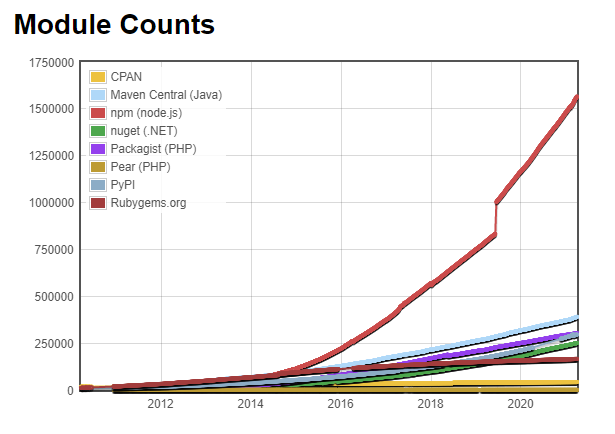
\includegraphics[width=0.7\textwidth]{obrazky-figures/modules.png}
	\caption{Porovnanie najpopulárnejších technológií a vývoj počtu ich modulov. Zdroj \cite{Moduleco}}
	\label{Moduleco_img}
\end{figure}

\bigskip

Pri porovnávaní technológií Puppeteer a Cheerio je na prvý pohľad jednoznačné čo majú spoločné, a v čom naopak každá z nich vyniká. Tieto poznatky pomôžu jednoznačne určiť technológiu na základe požiadavkov ktoré vznikli zároveň s výberom témy tejto práce.

Cheerio a Puppeteer sú technológie založené na Node.js, a patria medzi najpopulárnejšie technológie v tomto odvetví. Ich jednoznačné vlastnosti však definujú nielen ich možné prípady použitia, ale zároveň schopnosti a rýchlosť akou sú schopné dosiahnuť očakávané výsledky. 

Puppeteer je technológia ktorá je vyvíjaná za účelom automatizácie webového prehliadača, zatiaľčo hlavným určením Cheeria je web scraping samotný. Tým že je Cheerio určené priamo na požadovanú úlohu je v tomto ohľade rýchlejšie a výhodnejšie čo sa nášho požiadavku týka. Cheerio je zároveň multiplatformné, a dokáže pracovať ako s prehliadačom Firefox, tak s prehliadačom Google Chrome. Na druhú stranu Puppeteer je viazaný iba na prehliadač Google Chrome vo forme Chromium. Puppeteer má priamo kontrolu nad prehliadačom, takže je možné ovládať prehliadač ako celok. Tento fakt sa dá brať aj ako výhoda aj ako nevýhoda, keďže je to pravdepodobne jeden z dôvodov prečo je Puppeteer pomalší vo vykonávaní funkcie Web Scrapera. Puppeteer však prináša schopnosť plynulej práce s Javascriptom na webovej stránke, dokáže parsovať aj webové stránky postavené na moderných technológiách ako React alebo Angular, ktoré sú v dnešnej dobe na vzostupe pre ich moderné prvky. Z priamej integrácie s prehliadačom vyplýva aj fakt že Puppeteer dokáže vytvárať snímky obrazovky počas načítavania a pracovania s webovou stránkou. Zároveň podporuje technológiu XML, a nerobí mu problém ako čítanie, tak ani parsovanie a priame spúšťanie Javascriptových funkcií. \cite{Differences}

Práve podpora dodatočných funkcií a možnosť parsovania dynamických stránok s Javascriptom ma presvedčili o rozširovaní poznatkov technológie Puppeteer, a jej následné využitie pri návrhu architektúry a implementácie výslednej aplikácie.

\chapter{Technológie}
\label{Technologie}

Táto kapitola sa zaoberá popisom technológií, modulov a prvkov, na základe ktorých bude následne zostavená aplikácia tak, aby bolo čo najefektívnejšie nielen jej využívanie, ale aj údržba. Zároveň treba brať v úvahu aj prívetivosť a jednoduchosť užívateľského vstupu, a formát, využiteľnosť a prenositeľnosť výstupných dát. 

K výberu týchto technológií boli využité poznatky z Kapitoly \ref{aktualny_pristup}, ktoré ďalej určovali smer návrhu a vývoja aplikácie.

\section{HTML}

Základným stavebným blokom každej webovej stránky je nepochybne HTML. HTML je skratka pre \textit{Hypertext Markup Language}, a už svojím názvom napovedá akú úlohu vo webových technológiách zohráva. 

HTML dokument sa skladá z elementov, ktoré sú predstavené v podobe takzvaných \textit{tagov}. Tieto tagy sú reprezentované pomocou znakov \textit{<>} a dovoľujú určovať typ a rozsah uvedeného obsahu. Tieto elementy môžu obsahovať zároveň rôzne ďalšie atribúty, ako napríklad trieda elementu, alebo identifikátor. Takéto atribúty sú potom využívané v technológiách ktoré s HTML dokumentami spolupracujú, ako napríklad CSS a Javascript.

Takéto dokumenty sú následne reprezentované vo webovom prehliadači, ktorý HTML dokumenty zobrazí zároveň s doplnkovými dokumentami ktoré určujú štylizáciu a správanie sa danej webstránky. HTML dokumenty samotné neobsahujú žiadnu štylizáciu, avšak typ elementu ktorý použijeme pre realizovaní určitého prvku je kritický, pretože udáva základné rozloženie obsahu ktorý element predstavuje.\cite{WhatisHTML}

\section{DOM}

Jazyk HTML nieje určený na programovacie účely, a preto je potrebné pri práci s webovými stránkami zvážiť aj technológiu DOM. DOM je skratka ktorá reprezentuje \textit{Document Object Model}. Predstavuje akési prepojenie medzi HTML a programovacím jazykom ktorý chce s webovou stránkou komunikovať. \cite{DOM}

Pri komunikácií s programovacím jazykom DOM reprezentuje stránku v dvoch hlavných podobách:

\begin{itemize}
    \item {Uzly}
    \item {Objekty}
\end{itemize}

Práve tento fakt nám ďalej dovoľuje s webovou stránkou interagovať a meniť jej obsah. Príkladom takéhoto využitia jazyk Javascript, ktorý bol vyvinutý za účelom vytvorenia dojmu interakcie užívateľa s webovou stránkou. 

DOM je zároveň veľmi dôležitý pri web scrapingu, keďže práve komunikácia s webovou stránkou na úrovni programovacieho jazyka je kľúčová pri extrahovaní požadovaných údajov z webových dokumentov. Takáto extrakcia je možná vďaka reprezentácií webovej stránky v objektovo orientovanej podobe.

\section{CSS}

CSS predstavuje istý jazyk, ktorý je používaný za účelom popisu štylizácie HTML dokumentov. CSS znamená \textit{Cascading Style Sheets}, kde Cascading predstavuje jedno z hlavným pravidiel tohto jazyka - štylizačné pravidlá majú určenú prioritu podľa ktorej budú aplikované, a zároveň umožňujú na jednej webovej stránke používať viacero CSS súborov. 

Primárne určenie je už spomínaná štylizácia a definovanie rozloženia elementov na webovej stránke. Zároveň môžu definovať vzhľad v závislosti od zariadenia ktoré webovú stránku v danom momente navštívilo. 

HTML samotné nebolo vyvinuté za účelom definovania vzhľadu, a preto bolo nutné vyvinúť technológiu ktorá tento nedostatok kompenzovala. CSS pravidlá sú zväčša aplikované na atribút triedy, ktorý bliežšie špecifikuje skupinu prvkov v HTML dokumente. V niektorých prípadoch sa však pravdilá aplikujú aj na celé elementy, prípadne identifikátory.\cite{CSSIntro}

Pri vytváraní CSS pravidiel rozlišujeme 3 hlavné miesta kde sa tieto pravidlá môžu nachádzať:

\begin{itemize}
    \item {Riadkové}
    \item {Interné}
    \item {Externé}
\end{itemize}

Rozlišovanie medzi týmito typmi je dôležité, pretože z názvu \textit{Cascading} vyplýva že každé miesto môže mať inú prioritu finálneho vykonania daného pravidla.

\section{Javascript}

Programovací jazyk Javascript bol vyvinutý za účelom vytvárania dojmu interakcie pri webových stránkach. Javascript je jednou z hlavných súčastí webových stránok, a je používaný na viac ako 95\% stránkach celosvetovo.\cite{HowPopular} Dá sa preto predpokladať že bude jeho integrácia s webovými prehliadačmi a webovými stránkami na vysokej úrovni.
\newpage
Práve kombinácia HTML, CSS a Javascriptu totiž dokáže docieliť výsledky ktoré sa pri moderných štandardoch vyžadujú. Či už sa jedná o dynamickú zmenu obsahu alebo animovanie niektorých elementov, je to práve Javascript ktorý túto interakciu docieľuje. \cite{Javascript}

\begin{figure}[hbt]
	\centering
	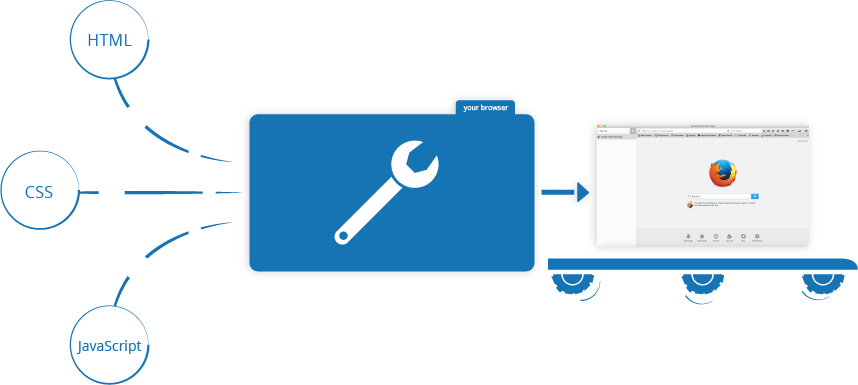
\includegraphics[width=0.5\textwidth]{obrazky-figures/jsexecution.png}
	\caption{HTML, CSS a JavaScript sú 3 hlavné zložky ktoré spolu vytvárajú web ako ho poznáme dnes. Zdroj \cite{Javascript}}
	\label{Jsexecution_img}
\end{figure}

\bigskip

Javascript je založený na programovacom jazyku Java, ktorý bol ďalej modifikovaný a prispôsobený na prácu priamo vo webovom prehliadači. Javascript dokáže nielen reagovať na vstupy od užívateľa, ale reagovať aj na niektoré udalosti ktoré sa stanú na pozadí, v prehliadači. \cite{Javascript}

Táto technológia ďalej stavia aj na asynchrónnosti, teda prístupu za behu. To dovoľuje stránkam načítať Javascript až po načítaní webového obsahu tak, aby nevznikali zbytočné dlhé čakacie doby na načítanie webstránky. Zároveň sa dá asynchrónnosť využiť pri odosielaní formulárov, kde nieje nutné po odoslaní znova načítavať stránku. Tým sa zároveň zlepšuje responzívnosť, keďže nieje nutné čakať na vykonanie špecifickej akcie. 

Jednou z najpopulárnejších vlastností tohto programovacieho jazyka je podpora API\footnote{Application Programming Interfaces}. Podpora API umožňuje využitie naprogramovaných rozhraní bez toho aby si tieto rozhrania užívateľ programoval sám. Tento fakt urýchľuje vývoj webových aplikácií a pomáha udržiavať štandard. API pri Javascripte sa primárne rozdeľujú do dvoch kategórií:

\begin{itemize}
    \item {Prehliadačové API}
    \item {Externé API}
\end{itemize}

Kde prehliadačové API predstavuje napríklad aj spomínaný DOM, ktorý javascriptu poskytuje HTML elementy vo forme objektov, s ktorými javascript dokáže pracovať. Čo sa externých API týka, sem patria najmä API tretích strán, ako napríklad Google Maps alebo Twitter.

V mnohých prípadoch sú to práve API, ktoré môžu naraziť na väčšie množstvo problémov pri načítavaní webovej stránky. Prispieva k tomu aj asynchrónnosť, kde v prípade že sa HTML dokument načíta skôr ako Javascriptové súbory, môže nastať problém kde vykonávanie skriptu zlyhá. Asynchrónnosť zároveň súvisí s postupnosťou vykonávania kódu. V prípade že je využitá asynchrónna funkcia, jej výsledok je reprezentovaný v podobe \textit{Promise}. Výsledok Promise nemusí byť dostupný okamžite, a preto v prípadoch že sa na túto skutočnosť neberie ohľad môže vykonávanie funkcie zlyhať.\cite{Javascript}

\newpage
\subsection{JSON}

Objekty sú v Javascripte popísané pomocou formátu JSON. JSON je skratka pre \textit{JavaScript Object Notation} kde už z názvu vyplýva jeho pôvod. Je to jednoduchá forma popisu objektov tak, že je vo výsledku ľahko čitateľná človekom, a zároveň jednoducho parsovatelná počítačom. \cite{JSON}

Aj keď je súčasťou názvu \textit{Javascript}, JSON je univerzálny spôsob zápisu objektov a je to formát adaptovaný mnohými programovacími jazykmi súčasnosti. Práve tieto vlastnosti robia z tohto formátu multiplatformný spôsob prenosu informácií.\cite{JSON}

\bigskip

JSON ponúka dve základné štruktúry:
\begin{itemize}
    \item {Objekt}
    \item {Pole}
\end{itemize}
Tieto základné štruktúry sú podporované modernými prehliadačmi a programovacími jazykmi ktoré sa v tomto zmysle používajú.\cite{JSON}

\subsection{Node.js}

Node.js ako runtime Javascritu bol vytvorený hlavne za účelom spracovávania asynchrónnych aplikácií. Beží na Javascriptovom rozhraní V8 ktoré bolo pôvodne vytvorené pre webový prehliadač Google Chrome. Práve vytvorenie tohto rozhrania viedlo k neskoršiemu vytvoreniu Node.js, pretože toto rozhranie dokázalo urýchliť Javascript kód pomocou priamej interpretácie tohto kódu do jazyku počítača. Node.js ako runtime predstavoval možnosť spúšťania Javascriptového kódu mimo webového prehliadača, priamo na fyzickom počítači. To viedlo k vytváraniu aplikácií priamo spustiteľných či už na počítači alebo smartfóne. Neskôr sa pridali rôzne moduly, ako napríklad HTTP, ktoré umožňovali ďalšie rozšírenie pôsobenia, a to napríklad aj na servery tak, aby mohol Node.js pôsobiť ako samostatné prostredie na strane servera. Node.js je v dnešnej dobe využívané zároveň pri technológiách ako napríklad React a Angular ktoré predstavujú frameworky založené a fungujúce práve vďaka Node.js.\cite{Node}

\bigskip

Node.js ponúka zároveň možnosť využitia rôznych modulov ktoré boli vyvinuté za účelom rozšírenia vlastností a funkcionality. Node.js sa aj vďaka týmto modulom a faktu že s jeho príchodom je možné Javascript využívať ako na backende tak aj na frontende stáva viac a viac populárnym. O tom svedčia aj jeho štatistiky z pohľadu vývoja týchto modulov. Moduly sú ďalej pre užívateľov distribuované pomocou NPM.

\subsection{NPM}

Jednou z najdôležitejších súčastí Node.js je NPM(Node Package Manager). Jedná sa o najväčšie a najpopulárnejšie úložisko doplnkových modulov a projektov pre Node.js. Jeho popularita stále stúpa a aktuálne sa v ňom nachádza už viac ako 1.5 milióna rôznych projektov \ref{Moduleco_img}\cite{npm}. A práve tu sa nachádza aj knižnica Puppeteer.

\newpage
\subsection{Puppeteer}

Hlavnou súčasťou výslednej aplikácie je Puppeteer. Je to jedna z mnoha knižníc vytvorených pre Node.js distribuovaná pomocou NPM. V aplikácií zohráva dôležitú úlohu, keďže práve technológia Puppeteer je spôsob akým aplikácia komunikuje a extrahuje údaje z prehliadača. 

Spojenie s prehliadačom je naviazané pomocou protokolu DevTools vyvinutého spoločnosťou Google, a používa prehliadač Google Chrome alebo Chromium v špeciálnom Headless móde, kedy nieje zobrazená vizuálna inštancia prehliadača, avšak všetky ostatné funkcie sú plne dostupné. \cite{puppeteer}

\bigskip

\begin{figure}[hbt]
	\centering
	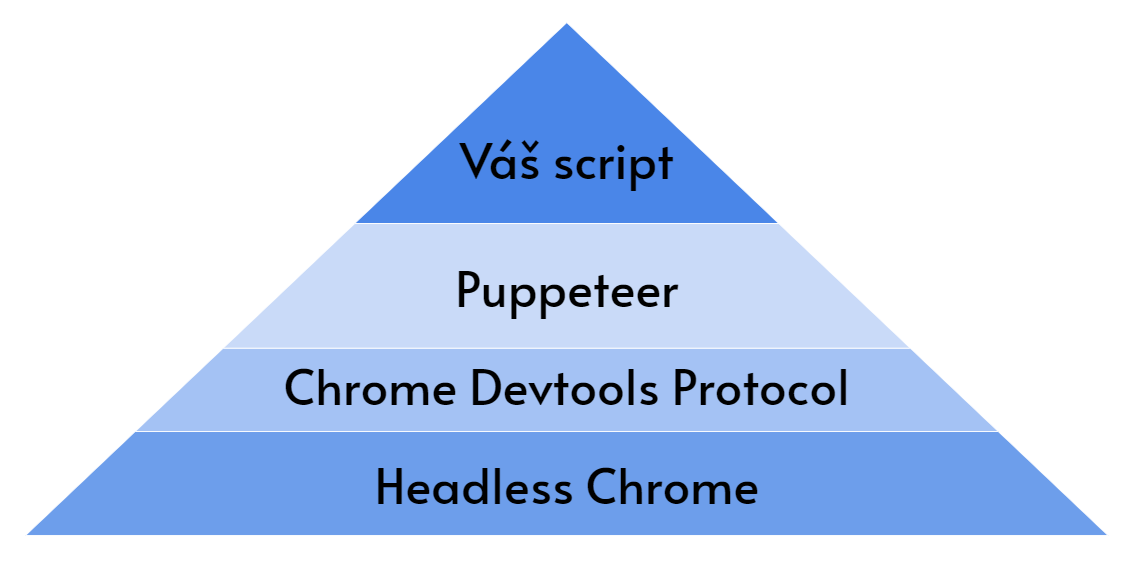
\includegraphics[width=0.5\textwidth]{obrazky-figures/puppepyramid.png}
	\caption{Hierarchia výslednej aplikácie pri použití technológie Puppeteer.}
	\label{pupepyramid_img}
\end{figure}

\bigskip

Z uvedenej hierarchie je na prvý pohľad jasné, na ktorých technológiách Puppeteer stavia:

\begin{enumerate}
  \item \textbf{Headless Chrome} je spôsob spustenia prostredia Chromium v takzvanom headless prostredí, kedy sa inštancia programu Google Chrome alebo Chromium spustí v režime server, bez užívateľského prostredia. Tento spôsob je pri používaní Puppeteeru nastavený ako základný, avšak je možné ho vypnúť a používať Chromium v headfull móde, teda so zobrazeným užívateľským prostredím.\cite{chromium}
  \item \textbf{Chrome DevTools protokol} bol založený za účelom automatizácie prehliadača Google Chrome, Chromium a ostatných webových prehliadačoch založených na prostredí Blink. Predstavuje komunikačný prvok medzi programom a webovým prehliadačom. Komunikačné kanály sú rozdelené podľa domén využitia a komunikácia medzi prehliadačom a aplikáciou ďalej prebieha využitím formátu JSON.\cite{devtools}
  \item \textbf{Puppeteer} ďalej nadväzuje na protokol DevTools v podobe API ktoré týmto protokolom dokáže komunikovať s inštanciou prehliadača Chrome. 
  \item \textbf{Váš script} následne využíva knižnicu Puppeteer ktorá prichádza s radom revolučných riešení umožňujúcich automatizovať takmer čokoľvek.
\end{enumerate}

\newpage

Puppeteer bol vytvorený za účelom kompletnej automatizácie správania prehliadača Google Chrome. Toto zahrňuje aj zber štatistík o používaní, a vykonávaní testov rôznych aplikácií.

Niektoré z ďalších prípadných využití tejto knižnice zahŕňajú aj:\cite{puppeteer}
\begin{itemize}
    \item {Vytváranie snímky obrazovky z webových stránok}
    \item {Automatizácia formulárov}
    \item {vytvorenie testovacieho prostredia pre akúkoľvek aplikáciu}
\end{itemize}

\bigskip

Online verzia Puppeteeru je zároveň dostupná v sandbox prostredí\footnote{\url{https://try-puppeteer.appspot.com/}} pre jednoduché vyskúšanie jeho možností.

\bigskip

Vo výslednej aplikácii je Puppeteer využívaný v rámci hlavného procesu, kde sa ako prvé vytvorí inštancia puppeteeru za pomoci príkazu \textit{await puppeteer.launch();} a následnom vytvorení inštancie stránky v podobe \textit{about:blank} za pomoci príkazu \textit{await browser.newPage();} ktorá následne slúži ako prostredie pre načítanie a následnú extrakciu dát z danej webovej stránky. Práca s knižnicou Puppeteer je napriek širokej škále funkcií jednoduchá.

\chapter{Návrh architektúry aplikácie}

Úlohou tejto kapitoly je oboznámenie s návrhom architektúry finálnej aplikácie. Architektúra sa skladá z definovaní požiadavkov na vstupné dáta, výstupné dáta a vnútorné chovanie aplikácie. V úvahu je samozrejme braná aj aktuálna situácia na trhu, a s tým spojená analýza ktorá určovala smer vývoja pri dôležitých otázkach ohľadne vnútornej štruktúry.

\section{Špecifikácia požiadaviek}

Ako už názov práce predpovedá, jedná sa o extrakciu dát z webových stránok. Avšak dáta sa z webových stránok dajú extrahovať mnohými spôsobmi, tie však niesu ekvivalentné. A to nielen z pohľadu presnosti, ale aj z pohľadu rýchlosti extrakcie, spôsobu extrakcie, a ďalších možnostiach ktoré sú viazané na spôsob aký je vo finálnej fáze zvolený.

Základom extrakcie je zároveň vedieť o aké dáta máme záujem. Tieto dáta teda musia byť jednou z hlavných častí ktoré budú definované na vstupe aplikácie. To v akom formáte a v akej podobe budú tieto dáta reprezentované bude popísané v nasledujúcich častiach tejto kapitoly. Už teraz je však isté, že pre dosiahnutie pomerne vysokej presnosti bude potrebná špecifikácia rôznych pravidiel. Tieto pravidlá potom budú udávať mernú jednotku na porovnávanie nájdených potencionálnych výsledkov s definovanými pravidlami.

Úlohou týchto pravidiel bude určenie relevantnosti nájdených dát. Aplikácia bude preto tieto vstupné pravidlá overovať z pohľadu správnosti formátu. Pri definícií týchto pravidiel bude treba pravdepodobne zohľadniť diverzitu a premenlivosť výsledného prvku, napríklad premenlivú dĺžku reťazcov. Dá sa teda s určitosťou predpokladať že správna definícia vstupných pravidiel bude mať jednoznačný vplyv na úspešnosť výsledkov z hľadiska nášho očakávania. Preto je treba tomuto návrhu venovať dostatočne veľký časový priestor.

Pri návrhu je treba samozrejme zohľadniť fakt, že finálny používateľ bude chcieť špecifikáciou týchto pravidiel stráviť čo najmenej času. To je samozrejmé, a je preto odlíšiť časti pravidiel ktoré nieje nutné prepisovať tak často od pravidiel ktoré sa môžu meniť s príchodom nových požiadaviek.

\newpage
\section{Vstupné pravidlá}

Pojmom vstupné pravidlá rozumieme pravidlá ktoré sú definované ako základné vstupné údaje pri spustení aplikácie. Tieto údaje budú mať za úlohu definovať presne to, čo v danom konkrétnom prípade užívateľ aplikácie očakáva ako aplikačný výstup. Sú to zároveň pravidlá pre aplikáciu, ktoré určujú objekty vo webovom dokumente určené na extrakciu.

Ako formát týchto pravidiel bol vybraný už spomínaný JSON, vďaka jeho jednoduchej zrozumiteľnosti ako z pohľadu človeka, tak aj z pohľadu počítača. Súbory vo formáte JSON sú zároveň veľmi jednoducho prenositelné aj medzi viacerými programovacími jazykmi, čo je samozrejme ďalšia výhoda. S týmto formátom mám zároveň osobné skúsenosti, takže to bola pomerne jasná voľba.

\subsection{Hlavné pravidlá}

V prvom rade treba začať prvotným upresnením, a teda z čoho sa vlastne tieto pravidlá budú skladať. S ohľadom na užívateľskú jednoduchosť, boli hlavné a vedľajšie pravidla rozdelené do dvoch konfiguračných súborov, pre ich jednoduchšiu správu. 

Medzi hlavné pravidlá na extrakciu boli vybraté:
\begin{itemize}
    \item {Zoznam webových stránok v podobe URL}
    \item {Štruktúra hľadaných prvkov}
    \item {Voliteľný atribút blacklist}
\end{itemize}

\bigskip

Kde \textbf{zoznam webových stránok} určuje všetky webové stránky ktoré sú určené na extrakciu. Budú to webové stránky ktoré budú ako atribút posielané aplikácii a výsledná aplikácia ich bude prechádzať v takom poradí, v akom boli zadané. V prípade že je niektorá zo stránok nedostupná, systém o tom užívateľa informuje, a bude pokračovať nasledovnou webovou stránkou. Pokračovanie namiesto ukončenia aplikácie je zvolené z dôvodu neustáleho vývoja webu. V prípade že jedna z preddefinovaných stránok zmení adresu, a táto adresa už nebude dostupná, by toto nemalo ovplyvniť vygenerovanie výsledkov ostatných adries.

\bigskip

\textbf{Štruktúra hľadaných prvkov} by mala byť definovaná ako objekt určujúci požadovaný výsledný názov elementu, teda jeho jednoznačný identifikátor, a jeho \uv{pseudo} dátový typ. Kde jeho identifikátor bude použitý zároveň pri finálnom výpise výsledných údajov, a dátový typ použitý podľa pravidiel ktoré budú popísané neskôr v tejto kapitole. Štruktúra je vo formáte objektu, a teda jednotlivé identifikátory a dátové typy sú k sebe priradené tak aby aj pre človeka bolo na prvý pohľad jasné v akom vzťahu tieto údaje sú.

\bigskip

\textbf{Blacklist} je voliteľný atribút (nemusí byť vo finálnom vstupnom súbore reprezentovaný). Predstavuje pole prvkov vo formáte reťazcov, ktoré užívateľ definuje ako také, ktoré by sa vo výslednom súbore nemali nachádzať. Definovanie takýchto reťazcov pomocou Blacklistu bude samozrejme mať za následok ovplyvnenie aplikácie pri rozhodovaní o pozícii a formáte výsledných údajov. 

\newpage
\subsection{Vedľajšie pravidlá}

Ako vedľajšie pravidlá boli zvolené také pravidlá, ktorých prenositeľnosť aj medzi rôznymi typmi definovaných domén je pravdepodobnejšia, a preto by nemuselo byť vždy nutné tieto pravidlá meniť. Zmena týchto pravidiel sa teda berie ako menej častá udalosť, a vo väčšine prípadov môže stačiť definovať hlavné pravidlá. 

Medzi tieto pravidlá boli zaradené:
\begin{itemize}
    \item {Maximálny pomer zlyhania}
    \item {Formát}
    \item {Primárny prvok}
\end{itemize}

\bigskip

Ako \textbf{maximálny pomer zlyhania} je určený výsledný pomer nesprávnych prvkov ku všetkým nájdeným prvkom z daného testovacieho okruhu. V prípade že je tento pomer vyšší ako definovaný je aktuálny testovací okruh zahodený a test prebieha nanovo s novým testovacím okruhom. Tento testovací okruh je reprezentovaný dátami, ktoré sú porovnávané s primárnym prvkom. Ten určuje či aktuálny kontrolovaný prvok spĺňa regulárny výraz primárneho prvku. V prípade že ho spĺňa je prvok nezmenený, v prípade že ho nespĺňa je prvok nahradený výrazom \textit{NULL} ktorý v následnom výpočte poslúži ako súčet prvkov ktorých kontrola \uv{zlyhala}. 

V prípade že je aktuálny pomer zlyhania menší ako maximálny pomer zlyhania definovaný vo vstupnom súbore, je daný testovací okruh braný za správny, uloží sa identifikátor okruhu a aplikácia pokračuje ďalšími krokmi ako napríklad generovanie výsledkov.

\bigskip

\textbf{Formát} predstavuje objekt ktorý sa skladá z názvu definovaného dátového typu a jeho korešpondujúcej reprezentácie v podobe jednoznačného regulárneho výrazu. Na dátové typy v tomto objekte naväzuje štruktúra prvkov definovaných v hlavných pravidlách. Štruktúra využíva práve dané regulárne výrazy na overenie správnosti zaradenia výsledného prvku.

Dá sa predpokladať že správne definovaný regulárny výraz bude mať dramatický vplyv na výsledné dáta. V prípade že test daného prvku na predpokladaný regulárny výraz neprejde, nieje možné určiť jeho dátový typ a teda výsledný jednoznačný identifikátor. V takom prípade nieje možné garantovať zaradenie takéhoto prvku do výsledného súboru dát.

\bigskip

\textbf{Primárny prvok} je taký prvok, ktorý je určený ako prvok ktorý sa v objekte určenom na extrakciu opakuje, a je teda možné sa na jeho prezenciu spoliehať. Tento prvok definuje objekt, a je možné nejakú jeho deriváciu nájsť v každom objekte ktorého obsah chceme extrahovať. 

Jeho reprezentácia je znova v podobe regulárneho výrazu, avšak on samotný sa nemusí nachádzať v definovanej štruktúre ani formáte vstupných údajov. Aplikácia tento prvok využíva na prvotnú analýzu stránky ako takej, a na základe jeho prezencie v danom testovacom okruhu je posúdené či daný testovaný okruh je kandidátom na definíciu správnych výsledných objektov.

\newpage
\section{Výstupný formát}

Čo sa výstupného formátu týka, mal by byť znovu pokiaľ možno v univerzálnom formáte. Keďže sa dá predpokladať že extrahované dáta budú v prípade potreby použité, je vhodné zvoliť formát ktorý je podporovaný rôznymi aplikáciami a programovacími jazykmi.

Z toho dôvodu tu bol znovu zvolený formát JSON. Návrh počíta s jedným výstupným súborom pre jednu doménu tak, aby výstupný súbor niesol názov domény z ktorej extrahované údaje pochádzajú. Umiestnenie týchto výsledných súborov je už však na užívateľovi, avšak pri nešpecifikovaní parametra určujúceho cestu k výstupným súborom bude použitá základná zložka s názvom \textit{output}.

\bigskip

Štruktúra v akej budú jednotlivé extrahované objekty reprezentované je zhodná so štruktúrou definovanou v užívateľskom vstupnom súbore. Táto štruktúra je potom zachovaná pre všetky objekty. Ak však nejaký kľúč z daného objektu nieje dostupný alebo nebol extrahovaný, je tento kľúč vynechaný. V niektorých prípadoch ak sa dátový typ daného prvku nepodarí overiť, a konfigurácia aplikácie je spustená bez parametru ktorý zaručuje odstránenie nedefinovaných prvkov z objektu, sa v objekte môžu nachádzať kľúče so špeciálnym názvom \textit{undefined}. Tento názov značí prvok, ktorého dátový typ nebolo možné na základe špecifikovaných vstupných požiadavkov definovať, avšak patrí do vyhľadávanej podskupiny.

Formát JSON ako výstupný formát je striktne dodržaný a riadne formátovaný tak, aby bol jednoducho čitateľný aj pre človeka. Bezproblémové využitie dát z takto štruktúrovaného výstupu je preto garantované.

\bigskip

Sekundárnym výstupným súborom sú takzvané metadáta. Sú to dáta ktoré predstavujú rôzne vlastnosti popisujúce priebeh extrakcie ktorá prebehla pri danom spustení aplikácie. Metadáta sú znova pre jednoduchú prenositeľnosť vo formáte JSON, a jeho objekty obsahujú tieto údaje:

\begin{itemize}
    \item {Url adresa webového dokumentu}
    \item {Počet testovaných okruhov}
    \item {Odkaz na prvý nájdený objekt v podobe \textit{document.querySelectorAll}}
    \item {Počet výsledných objektov}
    \item {Čas potrebný na otestovanie okruhov}
    \item {Čas potrebný na uloženie výsledkov}
    \item {Čas potrebný na načítanie webového dokumentu}
\end{itemize}

\bigskip

Tieto metadáta môžu poslúžiť ako kontrola výsledných súborov a porovnanie časov potrebných na vykonanie určitých akcií. Metadáta sú generované pri každom spustení aplikácie, a ich obsah je prepisovaný tak, aby obsahoval vždy údaje o poslednom spustení.

\newpage

\subsubsection{Konzolový výstup aplikácie}

Aplikácia zároveň pri každom spustení a jej behu informuje užívateľa o aktuálne prevádzanej akcii. V režime bez vypisovania explicitných informácií aplikácia informuje o začatí exekúcie formou vypísania \textit{Execution stared}. Následne po skontrolovaní vstupných údajov informuje o začatí extrakcie vypísaním \textit{BEGIN PRIMARY EXTRACTION}. Následne sa vypisujú aktuálne URL, na ktorých extrakcii sa v danom momente pracuje. 

Na záver aplikácia informuje o úspešnosti extrakcie, o lokácii vygenerovaného súboru s metadátami a o finálnej dĺžke trvania celého procesu v milisekundách.

V prípade spustenia programu s prepínačom \textit{-v} je na výstup vypísaný podrobnejší obsah. V tomto prípade sa na konzolovom výstupe objavia časy jednotlivých akcií, informácie o počte výsledných objektov a zoznam testovaných okruhov.

\section{Architektúra aplikácie}

V tejto časti práce bude popísaná architektúra aplikácie tak, ako bola aplikácia navrhnutá, a odôvodnenie týchto krokov. 

\subsection{Jadro programu}

Hlavný zdrojový kód sa bude nachádzať v jednom súbore ktorý pre jednoznačnosť v rámci tejto práce nazvem \textit{extractor.js}. Koncovka js napovedá že sa bude jednať o Javascriptový súbor. Pri spúšťaní aplikácie sa preto bude tento súbor volať pomocou príkazu \textit{node} ktorý značí Node.js.

Aplikácia bude naväzovať na dva prídavné súbory vo formáte JSON, ktoré budú predstavovať vstupné informácie vo formáte popísanom v predošlej časti tejto kapitoly. 

Hlavný komunikačný kanál aplikácie a webového prehliadača bude zabezpečený pomocou technológie Puppeteer a protokolu Chrome DevTools. Toto spojenie bude nadviazané automaticky po spustení aplikácie. Pred naviazaním tohto spojenia však dôjde ku kontrole vstupných dát zadaných používateľom. V prípade že je formát vstupných dát poškodený alebo nedodržaný, alebo vo vstupných súboroch chýbajú niektoré dôležité položky, je o tom používateľ informovaný a vykonávanie je ukončené.

\subsection{Hlavný proces}

Úlohou hlavného procesu bude vymedzenie finálneho okruhu výsledkov. Čo sa týchto okruhov týka, ich výber prešiel rôznymi iteráciami, avšak nakoniec bol zvolený spôsob určovania týchto okruhov na základe atribútu \textit{class}. Aplikácia teda najskôr analyzuje stránku tak, aby 
